\subsection{Recombination Factor}
%In this analysis, we use parameters of the Recombination factor in a measurement of Ref.\cite{658352}.
 Electron-ion recombination depends on the electric field and stopping power $dE/dx$. We study this factor using tagged proton beam. Recombination factor measurement using proton beam is relatively easy because of stability of proton. This is why we used proton beam for this study as a first step.\\
  Expression for recombination can be derived 

\begin{equation}
  Q = A\frac{Q_{0}}{1+(k/E)\times(dE/dx)\times(1/\rho)}
\end{equation}

where $Q_{0}$ is initial ionization charge, $E$ is electric field, $dE/dx$ is energy deposit per distance, $\rho$ is density of liquid Argon, A and k are fit parameters. This formula can be rearranged like below:

\begin{equation}
  \frac{Q_{0}}{Q} = \frac{1}{A}+\frac{(k/E)(dE/dx)(1/\rho)}{A}
\end{equation}

The ratio of $Q_{0}/Q$ depends on stopping power $dE/dx$, so we determined fit parameter A and k using proton data and Monte Carlo simulation. In this analysis, we need $Q$, $Q_{0}$ and $dE/dx$ channel by channel. First, electric field $E$ was 200 V/cm in our test. Second, $Q$ is integrated charge in an anode readout channel. Third, $Q_{0}$ is integrated charge without recombination factor in an anode readout channel. And then, $dE/dx$ per an anode channel is determined with truth information of Monte Carlo simulation. Figure \ref{fadcDist1}, \ref{fadcDistMC}, \ref{fadcDistdEdx} show $Q$, $Q_{0}$, $dE/dx$ as a function of distance from stopped channel between 1 to 14 channel. $Q$ is obtained from data, $Q_{0}$ and $dE/dx$ are obtained from Monte Carlo simulation.
In many case, integrated charge in stopped channel are more affected by noise from next channel. This is the reason why we don't use information from stopped channel in this analysis. 

%ch by ch data distribution
\begin{figure}[!htb]
  \centering
  \centering
  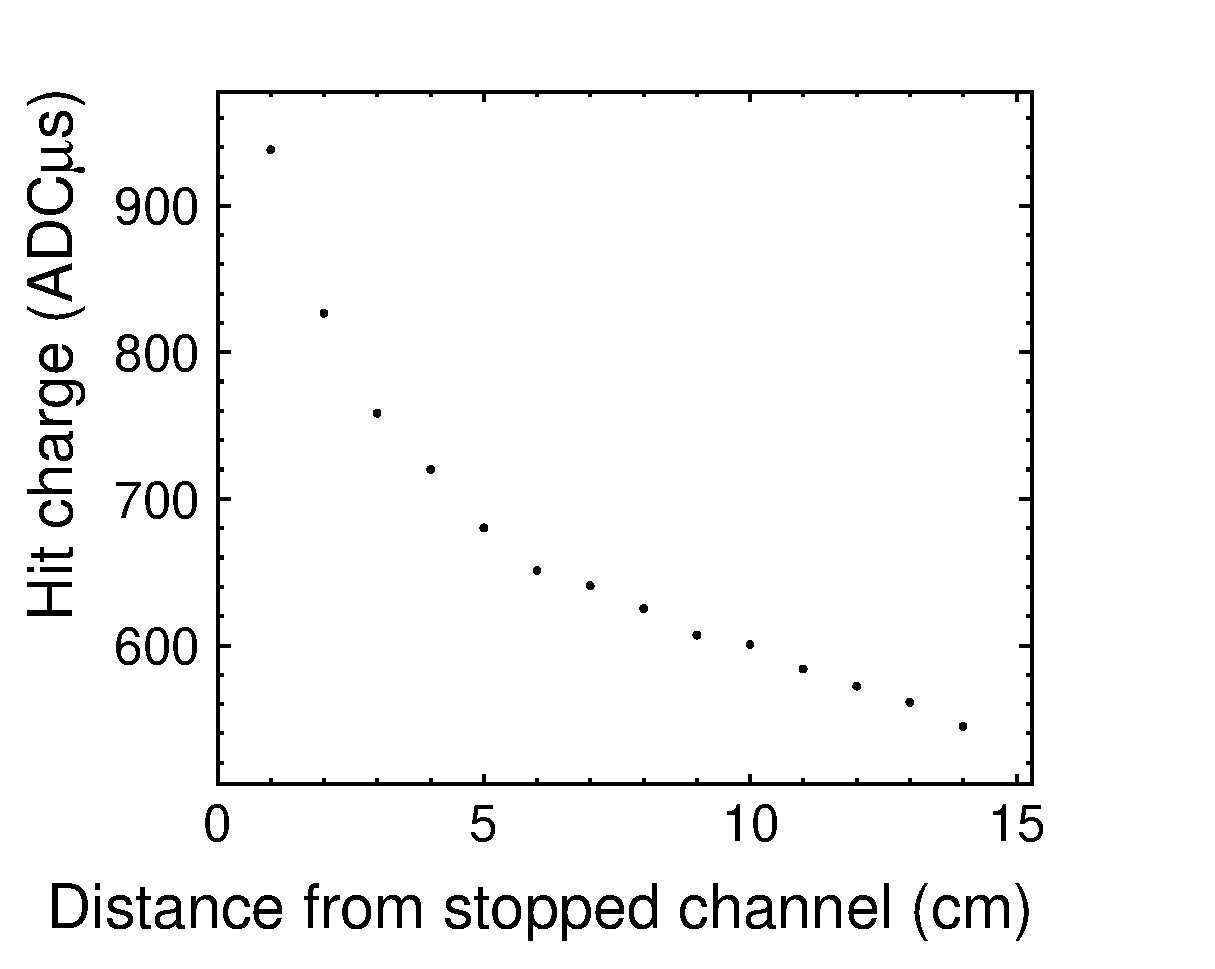
\includegraphics[width=10cm,clip]{./fig/Q2.eps}
%  \includegraphics[width=11cm,clip]{./fig/Data_FADCdistChbyCh.eps}
  \caption{DATA:Integrated Flash ADC counts from stopped channel -1}
  \label{fadcDist1}
\end{figure}
\pagebreak
\pagebreak

The result of this study is shown in Fig\ref{result}. Vertical axis is $Q_{0}/Q$, and horizontal axis is $dE/dx$ in this figure, this plot is fitted by Birks law.
As a result, we got fitting parameter\\
\begin{eqnarray}
%  \center
 \nonumber  A =& 0.832\pm0.009(stat.)\pm0.006(syst.)\\
   k =& 0.0504\pm0.0010 (stat.)\pm0.0013(syst.)\,(kV(g/cm^{2})/cm/MeV)
\end{eqnarray}

We checked Birks law in the range 4 $MeV/(g/cm^2)$ $\leqq dE/dx \leqq$ 12 $MeV/cm^2$ and the result is consistent with ICARUS experiment's one\cite{658352} in -- sigma.

%ch by ch MC distribution
\begin{figure}[!htb]
  \centering
  \centering
  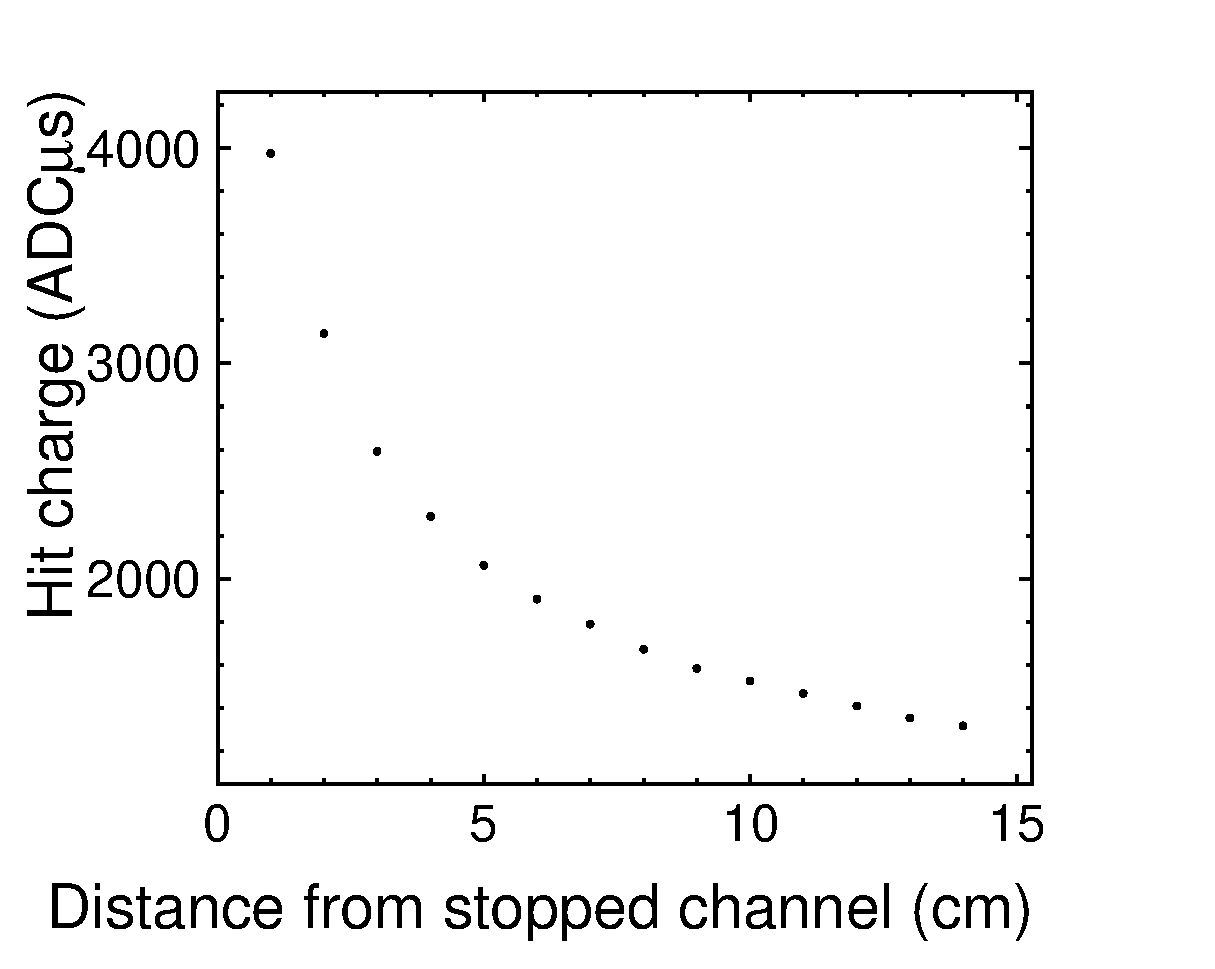
\includegraphics[width=10cm,clip]{./fig/Q_02.eps}
%  \includegraphics[width=11cm,clip]{./fig/MC_FADCdistChbyCh.eps}
%  \caption{MC:Distribution of Flash ADC counts ch by ch
  \caption{MC without recombination:Integrated Flash ADC counts from stopped channel -1}
  \label{fadcDistMC}
\end{figure}

%ch by ch dE/dx distribution
\begin{figure}[!htb]
  \centering
  \centering
  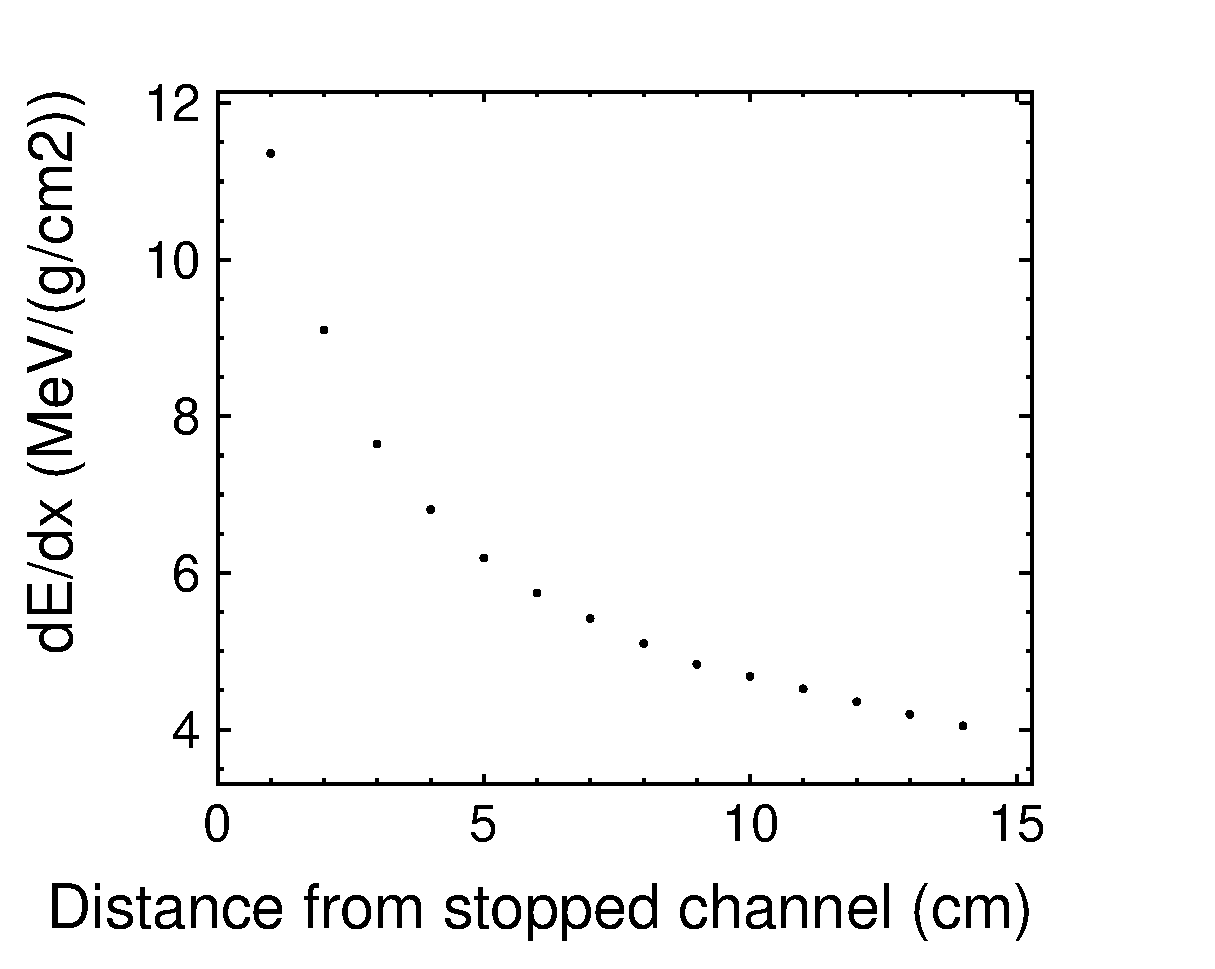
\includegraphics[width=10cm,clip]{./fig/dEdx2.eps}
%  \caption{Distribution of dE/dx ch by ch}
  \caption{dE/dx from stopped channel -1}
  \label{fadcDistdEdx}
\end{figure}

%result
\begin{figure}[!htb]
  \centering
  \centering
  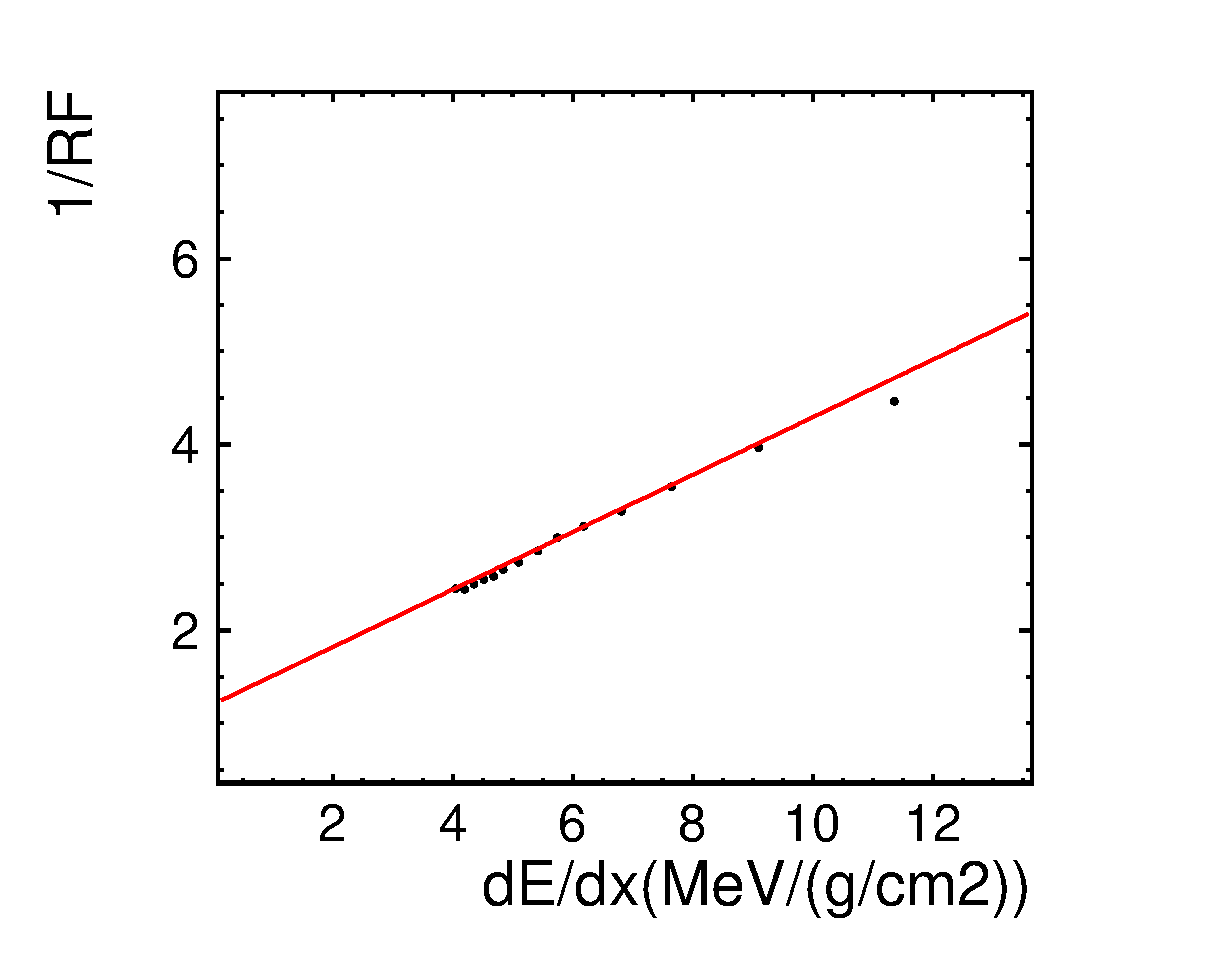
\includegraphics[width=10cm,clip]{./fig/RFresult2.eps}
  \caption{1/RF VS dE/dx: fitted by Birks law}
  \label{result}
\end{figure}

